%
\documentclass{research4cacm}
\usepackage{xspace}
\usepackage{fancyhdr,color,graphicx,epsfig} 
\usepackage{epsf}
\usepackage{epsfig}
\usepackage{latexsym}
\usepackage{dsfont}
\usepackage{url}
\usepackage{amsmath}
\usepackage{graphicx}
\usepackage{alltt}
\usepackage{url}
\usepackage{xspace}
\usepackage{floatflt}
\usepackage{wrapfig}
\usepackage{epsfig}
\usepackage{color,graphicx}
\usepackage{hhline}
\usepackage{alltt}
\usepackage{url}
%\usepackage{times}
%\usepackage{mathptmx}
\usepackage{xspace}
\usepackage{cite}
\usepackage{color}
\usepackage{epsfig}
\usepackage{theorem}

% Try to fill figures onto the page
\usepackage{amsmath,amssymb,amsfonts}
%\usepackage{times}
\usepackage{theorem}
\usepackage{color,graphicx}
\usepackage{boxedminipage}
\usepackage{program}
\usepackage{float}
\usepackage{array}
\usepackage{multirow}
\usepackage[tight]{subfigure}
\usepackage{fancyhdr}
\usepackage{calc}
%\usepackage{bibspacing}

\theoremstyle{plain}
\setlength{\theorempostskipamount}{5pt}
\setlength{\theorempreskipamount}{5pt}
%%%%%%%%%%%%%%%%%%%%%%%%%%%%%%%%%%%%%%%%%%%%%%%%%%%%%%%%%
\newtheorem{Def}{Definition}
\newtheorem{Not}{Notation}
\newtheorem{Claim}{Claim}
\newtheorem{Theorem}{Theorem}
\newtheorem{Lem}{Lemma}
\newtheorem{Cor}{Corollary}
\newtheorem{Example}{Example}
\newtheorem{Assumption}{Assumption}
\newtheorem{Constraint}{Constraint}
\providecommand{\LAR}{\leftarrow}
\providecommand{\RAR}{\rightarrow}
\providecommand{\DOT}{\centerdot}
\providecommand{\satisfies}{\rightarrow}


\floatstyle{ruled}
\newfloat{Algorithm}{thp}{lop}
\floatstyle{ruled}
\newfloat{Query}{thp}{lop}

\renewcommand{\topfraction}{1.00}
\renewcommand{\floatpagefraction}{1.00}
\renewcommand{\textfraction}{0.00}
\renewcommand{\dbltopfraction}{1.00}
\renewcommand{\dblfloatpagefraction}{1.00}

\def\ttt{~}
\def\mc{\prec_{mc}}
\def\po{\prec}
%\def\domain{\cal D}
\def\fc#1#2#3{#1 \mkern1mu\hbox{:}\; #2 \leadsto #3}
\def\mci#1#2#3{#1 \mkern1mu\hbox{:}\; #2 \prec_{mc} #3}
\def\eci#1#2#3{#1 \mkern1mu\hbox{:}\; #2 =_{ec} #3}
\def\Xvec{{\vec X}}
\def\Yvec{{\vec Y}}
\def\xvec{{\vec x}}
\def\yvec{{\vec y}}
\def\imp{\mathrel{:}\mathrel{-}}
\def\dcone{\bigvee_{i=1}^n {\cal C}_i}
\def\dctwo{\bigvee_{i=1}^m {\cal B}_i}
\def\edb{e_1,\ldots,e_m}
\def\comp{\circ}
\newcommand{\calp}{\ensuremath{\mathcal{P}}}
\newcommand{\calf}{\ensuremath{\mathcal{F}}}
\newcommand{\calc}{\ensuremath{\mathcal{C}}}
\newcommand{\caln}{\ensuremath{\mathcal{N}}}
\newcommand{\call}{\ensuremath{\mathcal{L}}}
\newcommand{\cala}{\ensuremath{\mathcal{A}}}
\newcommand{\calr}{\ensuremath{\mathcal{R}}}
\newcommand{\calv}{\ensuremath{\mathcal{V}}}
\newcommand{\calq}{\ensuremath{\mathcal{Q}}}
\newcommand{\calm}{\ensuremath{\mathcal{M}}}
%\newcommand{\tukwila}{\mbox{\sf Tukwila}}
\newcommand{\tukwila}{Tukwila}
%\newcommand{\Tukwila}{\mbox{\sf Tukwila}}
\newcommand{\Tukwila}{Tukwila}
\newcommand{\calo}{\ensuremath{\mathcal{O}}}
\newcommand{\calw}{\ensuremath{\mathcal{W}}}
\newcommand{\cals}{\ensuremath{\mathcal{S}}}
\newcommand{\calt}{\ensuremath{\mathcal{T}}}
\newcommand{\cale}{\ensuremath{\mathcal{E}}}
\newcommand{\cali}{\ensuremath{\mathcal{I}}}
\newcommand{\cald}{\ensuremath{\mathcal{D}}}
\newcommand{\calg}{\ensuremath{\mathcal{G}}}
\newif\iffullpaper
%\fullpaperfalse
\fullpapertrue


\newcommand{\ojoin}{\mbox{}^-_-\!\raisebox{-0.3mm}{$\bowtie$}\!^-_-}



%%%%%%%%%%%%%%%%  Weld's additions

\newcommand{\comment}[1]{}
\newcommand{\NOTE}[1]{\marginpar{\em {#1}}}
\newcommand{\bug}
    {\mbox{\rule{2mm}{2mm}}}
\newcommand{\Bug}[1]
    {\bug \footnote{BUG: {#1}}}
\newcommand{\TT}[1]{\mbox{\tt #1}}
\newcommand{\bi}{\begin{itemize}}
\newcommand{\ei}{\end{itemize}}
\newcommand{\BE}{\begin{enumerate}}
\newcommand{\EE}{\end{enumerate}}
\newcommand{\link}[1]{{\small \url{#1}}}


%\newcommand{\etc}{\mbox{\it etc.}}
%\newcommand{\eg}{\mbox{\it e.g.}}
%\newcommand{\ie}{\mbox{\it i.e.}}
%\newcommand{\Eg}{\mbox{\it E.g.}}
%\newcommand{\Ie}{\mbox{\it I.e.}}
%\newcommand{\etc}{\mbox{etc.}\xspace}
%\newcommand{\eg}{e.g.,}
%\newcommand{\ie}{i.e.,}
\newcommand{\?}{\mbox{?}}

\newcommand{\tuple}[1]
        {\mbox{$\langle{#1}\rangle$}}
%\newcommand{\set}[1]
%        {\mbox{$\{{#1}\}$}}
\newcommand{\size}[1]{\mbox{$\mid\!#1\!\mid$}}
\newcommand{\fun}[2]{$\mathbf{#1}(#2)$}

\newtheorem{defn}{Definition}
\newtheorem{them}{Proposition}          
\newtheorem{lemma}[them]{Proposition}   
%\newtheorem{example}{Example}
\newtheorem{ex}{Example}[section]



%%%%%%%%%%%%%%%%%% Friedman's additions

%\newcommand{\myps}[3]{\psfig{figure=#1,scale=100*{#2}}}
\newcommand{\myps}[3]{\rotatebox{#3}{\scalebox{#2}{\includegraphics{#1}}}}

%\newcommand{\myitem}[1] {{\noindent}{\bf {#1}}}
\newcommand{\myitem}[1] {\item {#1}}
\newcommand{\mylist}{\begin{itemize_squeeze}}
\newcommand{\mylistend}{\end{itemize_squeeze}}
\newcommand{\myparagraph}[1]{\vspace{-.15in}\paragraph{#1}}
\newcommand{\mysubsection}[1]{\vspace{-.1in}\subsection{#1}\vspace{-.12in}}
\newcommand{\mysubsubsection}[1]{\vspace{-.1in}\subsubsection{#1}\vspace{-.12in}}
\newcommand{\mysubsubsections}[1]{\vspace{-.1in}\subsubsection*{#1}\vspace{-.12in}}
\newcommand{\mycaption}[1]{\vspace{-.1in}\caption{#1}\vspace{-.13in}}
\newcommand{\mysection}[1]{\vspace{-.15in}\section{#1}\vspace{-.15in}}
%\newcommand{\pair}[2]   {\mbox{$\langle{\mbox{#1}},{\mbox{#2}}\rangle$}}
%\newcommand{\tuple}[1]   {\mbox{$\langle{\mbox{#1}}\rangle$}}
\newcommand{\triple}[3]{\ensuremath{(#1,#2,#3)}}
\newcommand{\pair}[2]{\ensuremath{(#1,#2)}}
\newcommand{\constant}[1]{\mbox{$\tt{#1}$}}
\newcommand{\etal}       {{\em et al.\/}}
\newcommand{\naive}      {na\"{\i}ve\xspace}
\newcommand{\Naive}      {Na\"{\i}ve}
\newcommand{\new}[1]{{\em #1\/}}                % New term (emphasized).
%\newcommand{\new}[1]     {\emph{#1}}
%\newcommand{\fixedfont}[1] {\texttt{#1}}
\newcommand{\fixedfont}[1]{#1} % fix this

\newenvironment{itemize_squeeze}{
  \begin{list}{$\bullet$}{
                \setlength{\rightmargin}{0pt}% Horizontal spacing
                \setlength{\listparindent}{0pt}
                \setlength{\itemindent}{0pt}
                \setlength{\labelwidth}{5pt}
                \setlength{\labelsep}{3pt}
                \setlength{\leftmargin}{8pt}
                \setlength{\parsep}{0pt}%        Vertical spacing
                \setlength{\itemsep}{0pt}
                \setlength{\topsep}{3pt}
                \setlength{\parskip}{0pt}
                \setlength{\partopsep}{0pt}}}
{
%                \addtolength{\textwidth}{1in}%               Misc
%                \addtolength{\oddsidemargin}{-.5in}
%                \addtolength{\textheight}{1.5in}
%                \addtolength{\topmargin}{-1in}
  \end{list}}

\newenvironment{itemize_squeeze_oneitem}{
  \begin{list}{ }{
                \setlength{\rightmargin}{0pt}% Horizontal spacing
                \setlength{\listparindent}{0pt}
                \setlength{\itemindent}{0pt}
                \setlength{\labelwidth}{5pt}
                \setlength{\labelsep}{3pt}
                \setlength{\leftmargin}{8pt}
                \setlength{\parsep}{0pt}%        Vertical spacing
                \setlength{\itemsep}{0pt}
                \setlength{\topsep}{3pt}
                \setlength{\parskip}{0pt}
                \setlength{\partopsep}{0pt}}}
{
  \end{list}}


%%%%%%%% Macros for examples, zives:
% \begin{example}{width}..\end{example} environment establishes minipage, 
%       increments ex. counter
% \begin{ecolumn}{width} creates a column with small font
%
% \ecaption{name}{text} creates a counter label plus a caption
% \eref{name} returns the counter value
\newcounter{example}
\newenvironment{example}[1][\textwidth]{\begin{minipage}[t]{#1}\addtocounter{example}{1}}{\end{minipage}}
\newenvironment{ecolumn}[1][3.5in]{\begin{minipage}[t]{#1}\footnotesize}{\end{minipage}}
\newcommand{\eref}[1]{\arabic{ex:#1}}
\newcommand{\ecaption}[2]{\center{Example \arabic{example}: #2}\vspace{+0.15in}\newcounter{ex:#1}\setcounter{ex:#1}{\arabic{example}}}

% Outputs a figure with a divider line at the top and bottom
\newenvironment{linedfig}{\begin{figure*}[tb]\rule{\textwidth}{0.5pt}}{\rule{\textwidth}{0.5pt}\end{figure*}}

% Use \openbox{\newcommandname} and \closebox{\newcommandname} (where \newcommandname is
% a command name you invent) to create a framed box into which you can put verbatim, etc.
% You can nest this inside of a figure environment, also (but the caption goes *outside*).
\newcommand{\openbox}[1]{\newsavebox{#1}\begin{lrbox}{#1}}
\newcommand{\closebox}[1]{\end{lrbox}\fbox{\usebox{#1}}}

\newcommand{\id}{{\tt ID}}
\newcommand{\idref}{{\tt IDREF}}
\newcommand{\idrefs}{{\tt IDREFS}}
\newcommand{\pcdata}{{\tt PCDATA}}

\newcommand{\appearedin}[1] {
\vspace{-2.5in}
\vbox to 0pt{\hfill\framebox{\bf \it Appeared in proceedings of #1}}
\vspace{2.5in}
}

\newcommand{\submittedto}[1] {
\vspace{-2.5in}
\vbox to 0pt{\hfill\framebox{\bf \it Submitted to #1}}
\vspace{2.5in}
}

\newenvironment{example2}{\begin{ex} \nopagebreak
  \begin{rm}}{{\hfill$\Box$}\end{rm}\end{ex}} 

\newenvironment{theorem}{\begin{thm} \nopagebreak}{\end{thm}}

\newenvironment{proof2}{\noindent {\bf Proof. } \nopagebreak 
\begin{normalsize}}{\end{normalsize}{\hfill$\Box$}\vspace*{0.2cm}}

\newenvironment{definition}[1]{\begin{defin}\begin{rm}({\bf 
#1})}{{\hfill$\Box$}\end{rm}\end{defin}}

\newenvironment{examp}{\begin{ex} \nopagebreak
  \begin{rm}}{{\hfill$\Box$}\end{rm}\end{ex}} 

\newenvironment{corollary}{\begin{corol} \nopagebreak}{\end{corol}}

\newenvironment{namedproof}[1]{\noindent {\bf Proof.}~(#1) \nopagebreak
\begin{normalsize}}{\end{normalsize}{\hfill$\Box$}\vspace*{0.2cm}}

\def\papernumber #1 raised #2 {
%\vspace{-#2}
\vbox to 0pt{\hfill\framebox{\bf \it Paper \# #1}}
\vspace{#2}
}

\def\dand{{\mbox{$\; \& \;$}}}
\def\dif{{\mbox{$\; :- \;$}}}
\def\tand{{\mbox{$\; \sqcap \;$}}}

\def\classic{{\sc Classic}}

\newcommand{\V}{\mbox{${\cal V}$}}
%\newcommand{\R}{\mbox{${\cal R}$}}
\newcommand{\barX}{{\bar X}}
\newcommand{\barY}{{\bar Y}}
\newcommand{\barA}{{\bar A}}
\newcommand{\barC}{{\bar C}}
\newcommand{\plan}{{\cal P}}
\newcommand{\query}{{\cal Q}}
\newcommand{\viewdef}{{\cal V}}
\newcommand{\vlit}{v}
\newcommand{\marker}{\star}
%\newcommand{\system}{``Q''}
\newcommand{\system}{Tukwila-CQP}

\newcommand{\eat}[1]{}

\newcommand{\reminder}[1]{{\bf  [[  #1 ]]}\typeout{#1}}



\def\Dlog{{\em NDlog}\xspace}
\def\Mlog{{\em Mozlog}\xspace}
\def\Overlog{{\em Overlog}\xspace}
\def\P2{{\em P2}\xspace}
\def\Pitu{{\em P2}\xspace}
\def\Sys{{\em P2}\xspace}
\newenvironment{SQL}{\begin{alltt}\footnotesize}{\end{alltt}}
\newcommand{\nd}[1]{\texttt{\scriptsize #1}}
\newenvironment{NDlog}{\vspace{-1.5mm}\begin{alltt}\scriptsize}{\end{alltt}\vspace{-1.5mm}}
\newcommand{\datalogspace}{\textcolor[gray]{1}{.}\hspace{0.8in}}
\newcommand{\lab}[1]{\textrm{\bf #1:\hspace{0.35in}}}

\newcommand{\jmh}[1]{\textcolor{red}{#1 -- jmh}}
\newcommand{\ion}[1]{\textcolor{blue}{#1 -- ion}}
\newcommand{\petros}[1]{\textcolor{green}{#1 -- petros}}

\newcounter{foo1}
\newenvironment{myenumerate}{\begin{list}{\arabic{foo1}.}{
      \usecounter{foo1}
      \setlength{\itemsep}{0mm}
      \setlength{\topsep}{0mm}
      \setlength{\itemsep}{-2pt}
}}{ \end{list}}

\def\PChordLines{48\xspace}
\def\PNaradaLines{16\xspace}

\linespread{1}
\begin{document}

\title{Declarative Networking}
%\thanks{The original version of this paper is entitled ``XXX" and was
%published in (Title of publication, publication date, publisher.)}
%}
%\subtitle{[Extended Abstract]
%\titlenote{A full version of this paper is available in...}
%}
%
% You need the command \numberofauthors to handle the 'placement
% and alignment' of the authors beneath the title.
%
% For aesthetic reasons, we recommend 'three authors at a time'
% i.e. three 'name/affiliation blocks' be placed beneath the title.
%
% NOTE: You are NOT restricted in how many 'rows' of
% "name/affiliations" may appear. We just ask that you restrict
% the number of 'columns' to three.
%
% Use the \alignauthor commands to handle the names
% and affiliations.
%

\numberofauthors{1} %  in this sample file, there are a *total*
\author{
\alignauthor Boon Thau Loo \quad Tyson Condie \quad Minos Garofalakis \quad David E. Gay\\
\vspace{0.05in}
Joseph M. Hellerstein \quad Petros Maniatis \quad Raghu Ramakrishnan\\
\vspace{0.05in}
Timothy Roscoe \quad Ion Stoica\\
\vspace{0.05in}
\fontsize{10}{10}\selectfont\itshape
\vspace{0.05in}
University of California-Berkeley \quad University of Pennsylvania \quad
Intel Research Berkeley\\
ETH Zurich \quad Yahoo Research \quad Technical University of Crete\\
\vspace{0.05in}
\fontsize{9}{9}\selectfont\ttfamily\upshape
boonloo@cis.upenn.edu \quad \{tcondie,hellerstein,istoica\}@cs.berkeley.edu \quad minos@softnet.tuc.gr\\
\{david.e.gay,petros.maniatis\}@intel.com \quad ramakris@yahoo-inc.com \quad troscoe@inf.ethz.ch
}

\eat{
\numberofauthors{9} %  in this sample file, there are a *total*
% of SIX authors and all of them fit neatly on the first page.  As said,
% all authors get 'equal billing' and you should fit all of them on the
% opening page in the 'byline'. The production/editorial-staff will
% 'separate' names from their affiliations, leaving author names beneath
% the title (in the byline), and moving the affilations/contact
% information to an area after the references at the back of the
% article.
%
\author{
% You can go ahead and credit any number of authors here,
% e.g. one 'row of three' or two rows (consisting of one row of three
% and a second row of one, two or three).
%
% The command \alignauthor (no curly braces needed) should
% precede each author name, affiliation/snail-mail address and
% e-mail address. Additionally, tag each line of
% affiliation/address with \affaddr, and tag the
% e-mail address with \email.
%
% 1st. author
\alignauthor
Boon Thau Loo\\
       \affaddr{University of Pennsylvania}\\
       \email{boonloo@cs.upenn.edu}
% 2nd. author
\alignauthor
Tyson Condie\\
       \affaddr{UC Berkeley}\\
       \email{tcondie@eecs.berkeley.edu}
% 3rd. author
\alignauthor Minos Garofalakis\\
       \affaddr{Technical University of Crete}\\
       \email{minos@softnet.tuc.gr}
\and  % use '\and' if you need 'another row' of author names
% 4th. author
\alignauthor David E. Gay\\
       \affaddr{Intel Research Berkeley}\\
       \email{david.e.gay@intel.com}
% 5th. author
\alignauthor Joseph M. Hellerstein\\
       \affaddr{UC Berkeley}\\
       \email{hellerstein@cs.berkeley.edu}
\alignauthor Petros Maniatis\\
       \affaddr{Intel Research Berkeley}\\
       \email{petros.maniatis@intel.com}
\and  % use '\and' if you need 'another row' of author names
\alignauthor Raghu Ramakrishnan\\
       \affaddr{Yahoo Research}\\
       \email{ramakris@yahoo-inc.com}
% 6th. author
\alignauthor Timothy Roscoe\\
       \affaddr{ETH Zurich}\\
       \email{troscoe@inf.ethz.ch}
\alignauthor Ion Stoica\\
       \affaddr{UC Berkeley}\\
       \email{istoica@cs.berkeley.edu}
}
}



\maketitle
\begin{abstract}
To be added
\end{abstract}

% The classification Scheme, General Terms and Keywords are not appropriate for CACM so comment them out.



\section{Introduction}
%Our research is motivated by two hard problems in distributed systems.  First,
\wrm{show examples of the problems (not necessarily code) -- evolving state and unreliable communication}

%Distributing any system introduces nondeterminism.  For example, one may
%distribute a computation over many inexpensive, but unreliable, commodity
%machines (e.g. RAID).  The status of internet links and widely distributed
%nodes is inherently more unreliable than multiple cores on a single die, or
%multiple CPUs in a single computer.  

%We present {\bf \lang}, a foundation language for programming and
%reasoning about distributed systems.  

%We correct deficiencies in earlier attempts, and introduce a compelling notion
%of non-determinism in the language.  We specifically use non-determinism to
%reason about {\em when} a deduction becomes visible, including the possibility
%that the deduction will never be visible.  Programmers can constrain this
%non-determinism by using well-studied techniques in distributed systems, such as
%Lamport Clocks 


Traditional database systems are based on declarative query languages that
specify transformations as dataflows over an updatable store.  Such query
languages are either not expressive enough to capture common programming
constructs \wrm{like what?}, or are at best awkward to use in this fashion.
\wrm{todo: transition that explains Datalog's birth from these languages... I
don't know enough to write it} The family of logic-based database languages, of
which Datalog is the progenitor, represent expressive programming languages
that produce similar dataflow representations.  Datalog is purely deductive: a
program specifies the rules by which the derived relations are populated based
on a static database, which is never updated.  Recent programming language
research has explored the use of Datalog-based languages for expressing
distributed systems.  Because the state of any complex system evolves with its
execution, these efforts were forced to extend the Datalog model by admitting
updates, additions and deletions of the EDB.  Unfortunately, these previous
attempts were plagued with ambiguities about how and when state changes occur
and become visible, putting a heavy burden on the programmer to ensure even
simple properties, such as atomicity of updates over time.

In contrast to reasoning about state change procdurally, \lang observes
that this concept is intuitively expressed as invariants over {\em time}.  In
this work, we present a formal model of Datalog augmented with time extensions.
By reifying time as data an introducing it into the logic, \lang eliminates
previous ambiguities, ensures atomicity of updates and makes it possible to
express system invariants that can guarantee liveness properties, a key
challenge in building distributed systems.

\section{Language}
\label{sec:language}

% present ndlog first as in sigcomm paper
% talk about events, etc extensions for soft-state

In this section we present an overview of the Network Datalog
(\Dlog) language for declarative networking. The \Dlog language is
based on extensions to traditional Datalog, a well-known recursive
query language designed for querying graph-structured
data in a centralized database. \Dlog's integration of networking and
logic is unique from the perspectives of both domains.  As a network
protocol language, it is notable for the absence of any communication
primitives like ``send'' or ``receive''; instead, communication is
implicit in a simple high-level specification of data partitioning.
In comparison to traditional logic languages, it is enhanced to
capture typical network realities including link-level constraints on
communication (and hence deduction), and failure-tolerant semantics of
persistence.

In this section, we step through an example to illustrate the standard
execution model for Datalog, and demonstrate its close connections to
routing protocols, recursive network graph computations, and
distributed state management. We then describe the
\Overlog~\cite{declareOverlays} extensions to the \Dlog language that
support soft-state data and events.

  

\subsection{Introduction to Datalog}
\label{sec:language: Datalog}

We first provide a short review of Datalog, following the conventions in
Ramakrishnan and Ullman's survey~\cite{ramakrishnan93survey}. A Datalog
program consists of a set of declarative {\em rules} and an optional
{\em query}. Since these programs are commonly called {\em ``recursive
  queries''} in the database literature, we use the term ``query'' and
``program'' interchangeably when we refer to a Datalog program.

A Datalog {\em rule} has the form {\em p :- $q_{1}, q_{2}, ...,
  q_{n}$}., which can be read informally as ``$q_{1}$ and $q_{2}$ and
$ ... $ and $q_{n}$ implies p''. $p$ is the {\em head} of the rule,
and $q_{1}, q_{2}, ..., q_{n}$ is a list of {\em literals} that
constitutes the {\em body} of the rule.  Literals are either {\em
  predicates} over {\em fields} (variables and constants), or functions
(formally, \emph{function symbols}) applied to fields. The rules can refer to each other in a
cyclic fashion to express recursion. The order in which the rules are
presented in a program is semantically immaterial.  The commas
separating the predicates in a rule are logical conjuncts ({\em AND});
the order in which predicates appear in a rule body also has no
semantic significance, though most implementations %(including ours)
employ a left-to-right execution strategy. The {\em query} specifies
the output of interest.

The predicates in the body and head of traditional Datalog rules are
relations, and we refer to them interchangeably as predicates, relations
or tables.  In our work every relation has a {\em primary key}, which is
a set of fields that uniquely identify each tuple within the
relation. In the absence of other information, the primary key is the
full set of fields in the relation.

By convention, the names of predicates, function symbols and
constants begin with a lower-case letter, while variable names begin
with an upper-case letter.  Most implementations of Datalog enhance it
with a limited set of side-effect-free function calls including standard
infix arithmetic and various simple string and list manipulations
(which start with ``\nd{f\_}'' in our syntax). Aggregate constructs are 
represented as functions with field variables within angle brackets ($<$$>$).

 



\subsection{NDLog by Example}
\label{sec:language:firstExample}

We introduce \Dlog using an example program shown below that
implements the {\em Path-vector protocol}, which computes in a
distributed fashion, for every
node, the shortest paths to all other nodes in a network. The path-vector protocol is used as the base
routing protocol for exchanging routes among Internet Service
Providers.

% \jmh{why bother with nexthop in these examples?  also, perhaps we should consider more descriptive variable names?}
% \ion{I agree with Joe that we need better names.}

\begin{NDlog}
sp1 path(@Src,Dest,Path,Cost) :- link(@Src,Dest,Cost),
    P=f\_init(Src,Dest).
sp2 path(@Src,Dest,Path,Cost) :- link(@Src,Nxt,C1),
    path(@Nxt,Dest,P2,C2), C=C1+C2, Path=f\_concatPath(Src,P2). 
sp3 spCost(@Src,Dest,min<Cost>) :- path(@Src,Dest,Nxt,P,Cost).
sp4 shortestPath(@Src,Dest,Path,Cost) :- spCost(@Src,Dest,Cost), 
    path(@Src,Dest,Path,Cost).
Query shortestPath(@Src,Dest,Path,Cost).
\end{NDlog}


The program has four rules (which for convenience we label
\nd{sp1-sp4}), and takes as input a base (``extensional'') relation
\nd{link(Source, Destination, Cost)}.  Rules \nd{sp1-sp2} are used to
derive ``paths'' in the graph, represented as tuples in the derived
(``intensional'') relation \nd{path(Src,Dest,Path,Cost)}.  The \nd{Src} and \nd{Dest}
fields represent the source and destination endpoints of the path,
\nd{Nxt} is the next hop along the path \nd{Path} from \nd{Src} to node
\nd{Dest}. The number and types of fields in relations are inferred from
their (consistent) use in the program's rules.

Since network protocols are typically computations over distributed
network state, one of the important requirements of \Dlog is the
ability to support rules that express distributed computations. \Dlog
builds upon traditional Datalog by providing control over the storage
location of tuples explicitly in the syntax via {\em location
  specifiers}. Each location specifier is a field within a
predicate that dictates the partitioning of the table datathe .  To
illustrate, in the above program, each predicate in the \Dlog rules
has an ``\nd{@}'' symbol prepended to a single field denoting the
location specifier. Each tuple generated is stored at the address
determined by its location specifier. For example, all \nd{path} and
\nd{link} tuples are stored  at the address held in the first
field \nd{@Src}.

%\jmh{there were some out-of-date rule names here that I modified to
%  match the text above.  later we have other rule name
%  inconsistencies.  Boon should probably decide how he wants to
%  unify.}

Rule \nd{sp1} produces \nd{path} tuples directly from existing
\nd{link} tuples, and rule \nd{sp2} recursively produces \nd{path}
tuples of increasing cost by matching (or {\em unifying}) the
destination fields of existing links to the source fields of
previously computed paths. The matching is expressed using the
repeated ``\nd{Nxt}'' variable in \nd{link(Src,Nxt,C1)} and
\nd{path(Nxt,Dest,Nxt2,C2)} of rule \nd{sp2}. Intuitively, rule \nd{sp2} says
that ``if there is a link from node \nd{Src} to node \nd{Nxt}, and there
is a path from node \nd{Nxt} to node \nd{Dest}, then there is a path \nd{Path}
from node \nd{Src} to node \nd{Dest} via the next hop \nd{Nxt}''.
 
Given the \nd{path} relation, rule \nd{sp3} derives the relation
\nd{spCost(Src,Dest,Cost)} that computes the minimum cost \nd{Cost} for each
source and destination for all input paths. Rule
\nd{sp4} takes as input \nd{spCost} and \nd{path} tuples and then
computes \nd{shortestPath(Src,Dest,Nxt,Cost)} tuples that contain the next hop
along the shortest path from \nd{Src} to \nd{Dest} with cost
\nd{Cost}. Last, the {\em Query} specifies the output of interest to be
the \nd{shortestPath} table.


\subsection{Shortest Path Execution Example}
\label{sec:queryExec}

We step through an execution of the {\em shortest-path} \Dlog program
above to illustrate derivation and communication of tuples as the
program is computed. We make use of the example network in
Figure~\ref{SP example}.  Our discussion is necessarily informal since
we have not yet presented our distributed implementation strategies;
in the next section, we show in greater detail the steps required to
generate the execution plan.  Here, we focus on a high-level
understanding of the data movement in the network during query
processing.


\begin{figure}[ht]
\centering
  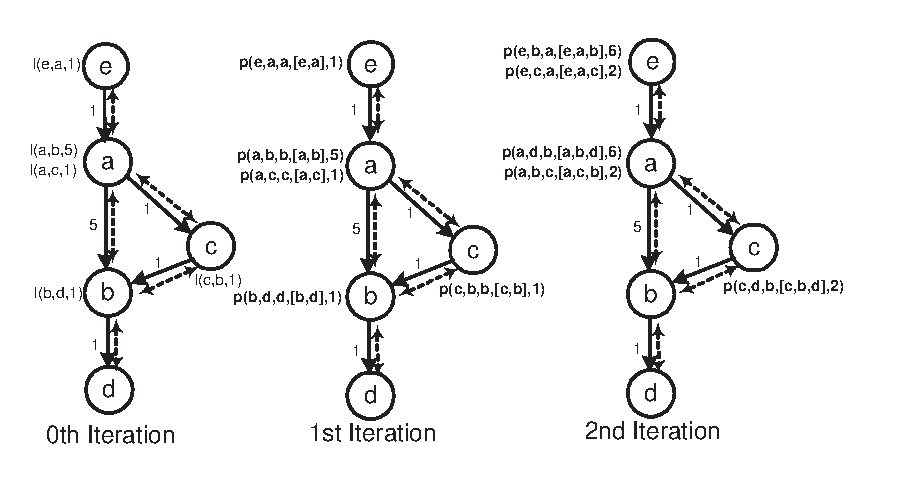
\includegraphics[width=3.5in]{graphs/example}
%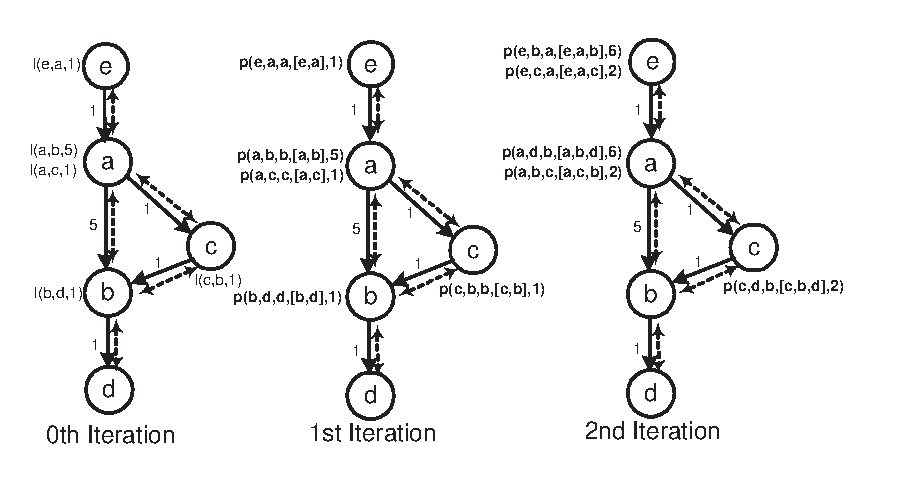
\epsfig{file=graphs/example., width=3.5in}
\caption{\label{SP example}{\small Nodes in the network are running
    the shortest-path query. We only show newly derived tuples at each
    iteration. For simplicity, we show only the derived paths along the
    solid lines even though the network connectivity is bidirectional
    (dashed lines).}}
\end{figure}                                              

For simplicity we will describe communication in {\em iterations}, where at each
iteration, each network node generates $paths$ of increasing hop
count, and then propagates these paths to neighbor nodes along
links. (We relax this notion in Section~\ref{sec:psn}.)  In the $1^{st}$ iteration, all nodes initialize their local
path tables to 1-hop paths using rule sp1. In the $2^{nd}$ iteration,
using rule sp2, each node takes the input paths generated in the
previous iteration, and computes 2-hop paths, which are then
propagated to its neighbors. For example, \nd{path(@a,d,[a,b,d],6)} is
generated at node {\em b} using \nd{path(@b,d,[b,d],1)} from the
$1^{st}$ iteration, and propagated to node {\em a}. In fact, many
network protocols propagate only the {\em nextHop} and avoid sending
the entire path vector.

%\jmh{Again, maybe we should leave out
%  nextHop?  Or instead say here that an alternative to passing paths
%  is to keep next-hops, which replaces the concat function with a
%  variable...?}

As paths are computed, the shortest one is incrementally
updated. For example, node $a$ uses rule sp1 to compute
\nd{path(@a,b,[a,b],5)}, and then sets its shortest path to
\nd{shortestPath(@a,b,[a,b],5)} using rule sp4. In the next iteration,
node $a$ receives \nd{path(@a,b,[a,c,b],2)} from node \nd{c} which has
lower cost compared to the previous shortest cost of 5, and hence
\nd{shortestPath(@a,b,[a,b],2)} replaces the previous tuple (the first
two fields of source and destination are the primary key of this relation).

Interestingly, while \Dlog is a language to describe networks, there
are no explicit communication primitives. All communication is
implicitly generated during rule execution as a result of data
placement specifications. For example, in rule \nd{sp2}, the \nd{path} and \nd{link}
predicates have different location specifiers, and in order to execute
the rule body of \nd{sp2} based on their matching fields, \nd{link}
and \nd{path} tuples have to be shipped in the network. It is the
movement of these tuples that will generate the messages for the
resulting network protocol.  


\subsection{Language Extensions}

We describe two extensions to the \Dlog language: {\em
  link-restricted rules} that limit the expressiveness of the
language in order to capture physical network constraints, and  
soft-state storage persistence commonly used in networking
protocols.

\subsubsection{Link-Restricted Rules}

In the above path vector protocol, the evaluation of a rule must
depend only on communication along the physical links.  In order to
send a message in a low-level network, there needs to be a link
between the sender and receiver. This is not a natural construct in
Datalog. Hence, to model physical networking components where
full connectivity is not available, \Dlog provides
restrictions ensuring that rule execution results in
communication only among nodes that are physically connected. This is
syntactically achieved with the use of the special \nd{link} predicate
in the form of {\em link-restricted rules}. A {\em link-restricted}
rule is either a local Datalog rule, or a rule with the following
properties:
\begin{myenumerate}
\item There is exactly one link predicate in the body
\item All other predicates (including the
      head predicate) have their
  location specifier set to either the first (source) or second
  (destination) field of the link predicate. 
\end{myenumerate}

This syntactic constraint precisely captures the requirement that we
be able to operate directly on a network whose link connectivity is
not a full mesh.  Further, as we demonstrate in
Section~\ref{sec:queryPro}, link-restriction also guarantees that all
programs with only link-restricted rules can be rewritten into a
canonical form where every rule body can be evaluated on a single
node, with communication to a head predicate along links. The following is an example of
a link-restricted rule:
\begin{NDlog}
p(@Dest,...) :- link(@Src,Dest...),p1(@Src,...),p2(@Src,...),
                ..., pn(@Src,...).
\end{NDlog}
The rule body of this example is executed at \nd{@Src} and the resulting $p$
tuples are sent to \nd{@Dest}, preserving the communication constraints along
links. Note that the body predicates of this example all have the same
location specifier: \nd{@Src}, the source of the link. In contrast, rule
\nd{sp2} of the \emph{shortest path} program is link-restricted but has some
relations whose location specifier is the source, and others whose
location specifier is the destination; this needs to be rewritten
to be executable in the network, a topic we return to in
  Section~\ref{subsec:ruleLocalization}. 
% While link-restricted rules
% limit the expressiveness of the permitted set of declarative networks,
% the restrictions enable us to better reason about eventual consistency
% of network protocols by placing constraints on FIFO link channels.
% \jmh{The material mentioned in the last
%   sentence is covered in \ref{subsec:ruleLocalization}, no?  Should we
%   try to move localization up here next to link restriction?  Seems
%   kind of natural.} \petros{I kind of like the current location of
%   localization. This is about language semantics. The localization section is
%   about query plan generation.}

Note that in a fully-connected network environment, an \Dlog parser can
be configured to bypass the requirement for link-restricted rules.


%See \cite{declareNetworks} for
%details.




%\reminder{Add a discussion on link-restricted rules. Proofs in SIGMOD paper}

\subsubsection{Soft-state Storage Model}
\label{sec:dn:softstate}

Many network protocols use the {\em soft-state}~\cite{clark88design}
approach to maintain distributed state. In the soft state storage
model, stored data have an associated {\em lifetime} or time-to-live
(TTL). A soft-state datum needs to be periodically refreshed; if more time
than a TTL passes without a datum being refreshed, that datum is deleted.  Soft
state is often favored in networking implementations because in a very
simple manner it provides well-defined eventual consistency
semantics. Intuitively, periodic refreshes to network state ensure
that the eventual values are obtained even if there are transient
errors such as reordered messages, node disconnection or link
failures.  However when persistent failures occur, no coordination is
required to register the failure: any data provided by failed nodes is
organically ``forgotten'' in the absence of refreshes.

We introduced soft-state into the \Overlog~\cite{declareOverlays}
declarative networking language, an extension of \Dlog. One additional
feature of \Overlog is the availability of a
\nd{materialized}~\cite{declareOverlays} keyword at the beginning of
each \Dlog program to specify the TTL of predicates. For example,
the definition \nd{materialized(link, \{1,2\}, 10)} specifies that the
\nd{link} table has its primary key set to the first and second
fields (denoted by \nd{\{1,2\}}),
% \footnote{Following the
  % conventions of the \Pitu declarative networking system, field 0
  % is reserved for the predicate name.} 
and each \nd{link} tuple has a
lifetime of 10 seconds.  If the TTL is set to infinity, the predicate
will be treated as {\em hard state}, i.e., a traditional relation that does not involve timeout-based deletion.

% \jmh{Hard state semantics are notably missing here.  I think you
%   should describe them w.r.t. local view materialization of Datalog.
%   You may also want to cite your thesis w.r.t, the subtleties of rules
%   that mix hard and soft state.  My group is still not sure how we
%   like to think about state updates for hard state, BTW.}

The \Overlog soft-state storage semantics are as
follows. When a tuple is derived, if there exists another tuple with
the same primary key but differences on other fields, an {\em update}
occurs, in which the new tuple replaces the previous one. On the other
hand, if the two tuples are identical, a {\em refresh} occurs, in
which the existing tuple is extended by its TTL.

If a given predicate has no associated \nd{materialize}
declaration, it is treated as an {\em event} predicate: a soft-state
predicate with TTL=0. Event predicates are transient tables, which are
used as input to rules but not stored. They are primarily used to
``trigger'' rules periodically or in response to network events. 
For example, utilizing \Overlog's
built-in \nd{periodic} event predicate, the following rule enables node \nd{X}
to generate a \nd{ping} event every 10 seconds to its neighbor \nd{Y}
denoted in the \nd{link(@X,Y)} predicate: 

\begin{NDlog}
ping(@Y,X) :- periodic(@X,10), link(@X,Y).
\end{NDlog}

Subtleties arise in the semantics of rules that mix event, soft-state
and hard-state predicates across the head and body.  One issue
involves the expiry of soft-state and event tuples, as compared to
deletion of hard-state tuples. In a traditional hard-state model,
deletions from a rule's body relations require revisions to the
derived head relation to maintain consistency of the rule.  This is
treated by research on materialized view
maintenance~\cite{rossMatviews}.  In a pure soft state model, the head
and body predicates can be left inconsistent with each other for a
time, until head predicates expire due to the lack of refreshes from
body predicates. Mixtures of the two models become more subtle.  We
provided one treatment of this issue~\cite{boonThesis}, which has
subsequently been revised with a slightly different interpretation
~\cite{evitaRaced}. There is still some debate about the desired
semantics, focusing around attempts to provide an intuitive
declarative representation while enabling familiar event-handler
design patterns used by protocol developers.

%and Navarro details the operational semantics
%embodied in a version of the P2 implementation~\cite{Navarro}. 


% 
% \jmh{Perhaps add a ``Discussion'' subsection that exposes some of the soft underbelly of our semantics.  One issue is that we allow ``hard-state'' tables in the heads of rules, whereas in  Datalog the heads are IDB tables (``views'').  IN some cases this is consistent with materialized view semantics (all hard state rules).  In others, it's more like ``insert'': we keep the tuples in those tables persistent even when the bodies don't support those tuples anymore (e.g. soft-state expiry, event tables).  Another issue: how do we model aggregation/negation w.r.t. delayed delivery of tuples?  There are more of these kinds of warts exposed in Navarro's paper on the ``operational semantics of declarative nets''.  }

\subsubsection{Additional Extensions of \Overlog}
\Overlog adds a number of features to \Dlog.  In addition to soft state, \Overlog adds support for negation and aggregation, including checks for stratification.  It also adds the ability to update the database via derivation of new facts to be inserted into database tables, as well as explicit deletion rules whose effects are deferred until after fixpoint.  \Overlog also provides a notion of unique keys for a relation, and the ability for the derivation of a new fact to ``overwrite'' a previous fact with a matching key.  State management and event handling semantics in \Overlog and related languages have been an evolving mix of declarative and operational notions~\cite{declareOverlays,dsn,navarro,evita,boom}, and are still a subject of active research.

%\section{Runtime System}

The execution model of declarative networks is based on a distributed
variant of the standard evaluation technique for Datalog programs that
is commonly known as {\em semi-\naive} (SN)
evaluation~\cite{declareNetworks}, with modifications to enable
pipelined asynchronous evaluation suited to a distributed setting.
Reference~\cite{declareNetworks} provides details on the implementation
and execution model of declarative networking.

Unlike traditional semi-\naive\ evaluation, PSN does not require
computations in synchronous rounds (or iterations), a prohibitively
expensive operation in distributed settings.  We consider the following
recursive Datalog rule:

% \begin{equation}\label{eqn:central}

%\vspace{-0.1in}
\begin{center}$d $ :- $ d_{1}, d_{2}, ..., d_{n}, b_{1}, b_{2}, ..., b_{m}$\end{center}
%\vspace{-0.1in}

\noindent where there are $n$ derived predicates ($d_{1},...,d_{n}$),
and $m$ {\em base predicates} ($b_{1},...,b_{m}$) in the rule body.
Derived predicates refer to intensional relations that are derived
during rule execution, and may be mutually recursive with $d$.  Base
predicates refer to extensional (stored) relations whose values are not
changed during rule execution.  In PSN, a delta rule is generated for
each derived predicate, where the $k^{th}$ {\em delta rule} is of the
form:
%\vspace{-0.1in}
\begin{center}$\triangle d$ :- $ d_{1},..,d_{k-1},\triangle d_{k}, d_{k+1},..,d_{n},
b_{1},b_{2},...,b_{m}$\end{center}

\noindent where $\triangle d_{k}$ denotes a tuple $t_{k} \in d_{k}$ that is used as
input to the rule for computing new $d$ tuples.

In the simplest version of PSN with no buffering, tuples are processed
tuple-at-time in a pipelined fashion.  Each node maintains a FIFO queue
(ordered by arrival timestamp) of new input tuples.  Each new tuple is
dequeued and is used as input to its respective a delta rule.  The
execution of a delta rule may generate new tuples which are either
inserted into the local queue or sent to a remote node for further
execution.  Duplicate evaluations are avoided using local arrival
timestamps, where each new tuple is only processed with tuples with
older timestamps.


\reminder{Add PSN, semi-naive evaluation, and localization rewrite via
  exmaple. Proofs in paper.}

\section{Execution Plan Generation}
\label{sec:queryPro}

Having illustrated the intended execution of an example program, we
now describe the steps required to automatically generate an execution plan from a
\Dlog program. We first focus on generating
an execution plan in a centralized implementation, before extending
the techniques to the network scenario.

\subsection{Centralized Plan Generation}
\label{sec:semiNaive}

In generating the centralized plan, we utilize the well-known {\em
  semi-\naive fixpoint}~\cite{semi,semi1} evaluation mechanism that
ensures no redundant evaluations. As a quick review, in semi-\naive (SN) evaluation, input
  tuples computed in the previous iteration of a recursive rule
  execution are used as input in the current iteration to compute
  new tuples. Any new tuples that are generated for the first time in the current
  iteration are then used as input to the next iteration. This is repeated until a
  fixpoint is achieved (\ie no new tuples are produced).

The semi-\naive rewritten rule for rule SP2 is shown below:

\vspace{2pt}
{\small
\noindent{\bf SP2-1: } $\triangle$path$^{new}$({\bf @S},@D,@Z,P,C) :- \link({{\bf @S},@Z},C$_{1}$),\\
\datalogspace
$\triangle$path$^{old}$({\bf @Z},@D,@Z$_{2}$,P$_{2}$,C$_{2}$), C = C$_{1}$ + C$_{2}$, \\                              
\datalogspace P =
$f\_concatPath$(link({{\bf @S},@Z},C$_{1}$),P$_{2}$).\\ 
}

\vspace{2pt}


%SP2-1* takes as input paths ($\triangle$path$^{old}$) computed in the previous
%invocation of the rule (known as an {\em iteration}), and use that to
%compute new paths ($\triangle$path$^{new}$). 


%Since links can also be modified during query execution, we need a
%similar rewrite for links (SP2-2). 

%{\small
%\noindent{\bf SP2-2: } $\triangle$path$^{new}$({\bf @S},@Z,@D,P,C) :-
%$\triangle$link({{\bf @Z},@S},C$_{1}$),\\
%\datalogspace path({\bf @Z},@D,@N,P$_{2}$,C$_{2}$), C = C$_{1}$ + C$_{2}$, \\                              
%\datalogspace P = $f\_concatPath$(linkD({\bf @Z},@S,C$_{1}$),P$_{2}$).\\ 
%}


\begin{figure*}[ht]
\centering
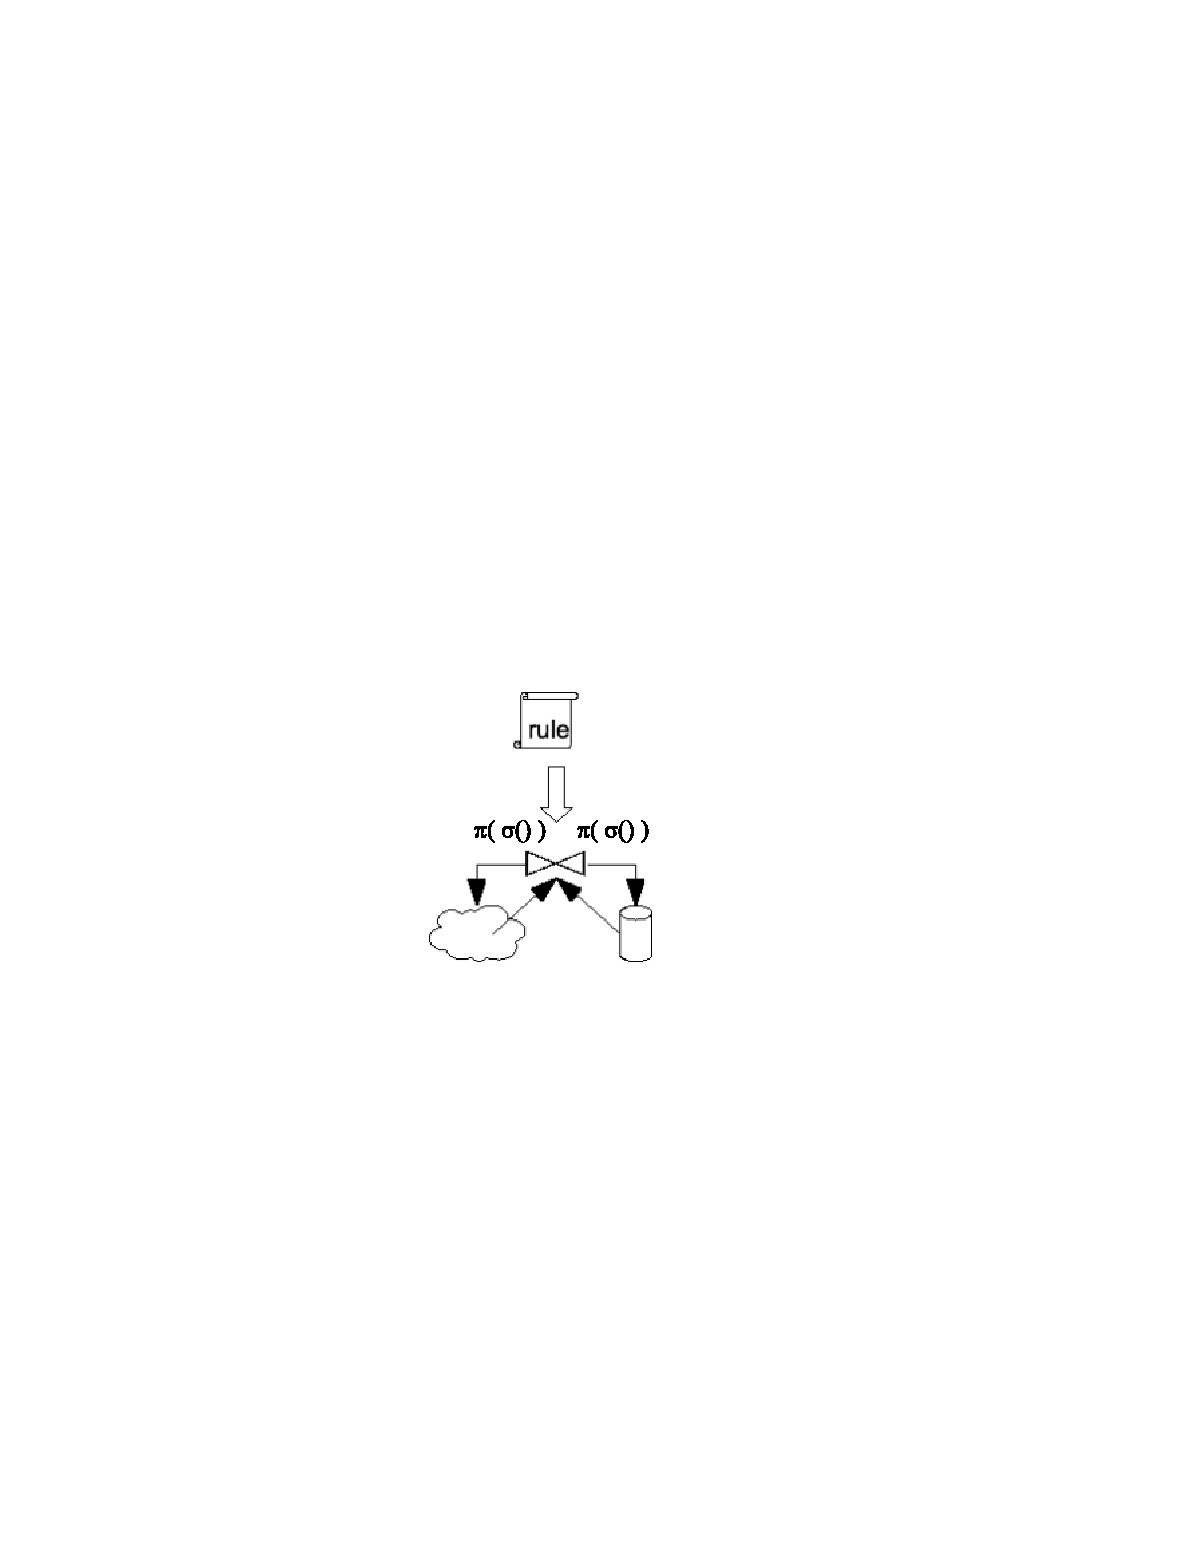
\epsfig{file=images/dataflow.eps, width=5in}
\caption{\label{Dataflow}\emph{\small Rule strand for rule SP2-1 in
    \Sys. Output paths that are generated from the strand are ``wrapped
    back'' as input into the same strand. }}
\end{figure*}                                        

Figure~\ref{Dataflow} shows the dataflow realization for rule SP2-1
using the conventions of \Sys. We will briefly explain how the semi-\naive evaluation is
achieved here. Each semi-\naive rule is implemented as a {\em rule strand}. Each strand
consists of a number of relational operators. The example strand
receives new $\triangle$$path^{old}$ tuples generated in the previous
iteration to generate new paths ($\triangle$$path^{new}$) which are
then inserted into the $path$ table (with duplicate elimination) for
further processing in the next iteration. 

In Algorithm~\ref{alg:sn}, we show the pseudocode for a centralized
\Sys implementation of multiple semi-\naive
rule strands where each rule has the form $\triangle$p$^{new}_{j}$ :-
$p^{old}_{1}$,..., $p^{old}_{k-1}$,$\triangle$p$^{old}_{k}$,$p_{k+1}$,...,$p_{n},b_{1},
b_{2},...,b_{m}$;\footnote{These rules are logically equivalent to rules
  of the form $\triangle$p$^{new}_{j}$ :- $p_{1},p_{2}$,...,$p_{k-1}$,$\triangle$p$^{old}_{k}$,$p_{k+1}$,...,$p_{n},b_{1},b_{2},...,b_{m}$,
  and have the advantage of avoiding redundant inferences within each iteration.}
\\$p_{1},...,p_{n}$ are recursive predicates and $b_{1},...b_{m}$ are base
predicates. $\triangle$p$^{old}_{k}$ refers to $p_{k}$ tuples generated
for the first time in the previous iteration. $p^{old}_{k}$
refers to all $p_{k}$ tuples generated before the previous iteration.

%|\quad | \triangle 
\vspace{2pt}
\begin{Algorithm}[ht]
  \begin{programbox}
%    |Initialize all | p_{i} | and | \triangle p^{new}_{i} to | null |
    \WHILE \exists B_{k}.size > 0
     \forall B_{k} | where | B_{k}.size > 0, \triangle p^{old}_{k} \leftarrow B_{k}.flush()
	|execute all rule strands | 	
	\FOREACH | recursive predicate | p_{j} 
	  p^{old}_{j} \leftarrow p^{old}_{j} \union \triangle p^{old}_{j}
	  B_{j} \leftarrow \triangle p^{new}_{j} - p^{old}_{j}
	  p_{j} \leftarrow p^{old}_{j} \union B_{j}
	  \triangle p^{new}_{j} \leftarrow \emptyset
%	\END
%    \END	      
\end{programbox}
\caption{Semi-\naive (SN) Evaluation in \Sys}
\label{alg:sn}
\end{Algorithm}
%end{boxedminipage}
\vspace{2pt}

In the algorithm, $B_{k}$ denotes the buffer for $p_{k}$ tuples
generated in the previous iteration
($\triangle$$p^{old}_{k}$). Initially, $p_{k}$, $p^{old}_{k}$, $\triangle$$p^{old}_{k}$ and
$\triangle$$p^{new}_{k}$ are empty. As a base case, we
execute all the rules to generate the initial $p_{k}$ tuples, which
are inserted into the corresponding $B_{k}$ buffers.  Each subsequent
iteration of the while loop consists of flushing all
existing $\triangle$$p^{old}_{k}$ tuples from $B_{k}$ and executing all
rule strands to generate $\triangle$$p^{new}_{j}$ tuples, which are used
to update $p^{old}_{j}$, $B_{j}$ and $p_{j}$ accordingly. Note that only new $p_{j}$ tuples
generated in the current iteration are inserted into $B_{j}$ for use in
the next iteration. Fixpoint is reached when all buffers are empty.
 
\subsection{Distributed Plan Generation}
\label{subsec:ruleLocalization}

In the distributed implementation of the {\em shortest-path} query,
non-local rules whose body predicates have different location
specifiers cannot be executed at a single node, since the tuples that
must be joined are situated at different nodes in the network. A {\em
  rule localization} rewrite step ensures that all tuples to be joined
are at the same node. This
allows a rule body to be locally computable.

%This step requires
%determining a distributed join ordering for predicates at different
%locations. 


\begin{figure}[ht]
\centering
\includegraphics[width=2.5in]{images/reachable.eps}
\caption{\label{Right Reachable}\emph{\small Logical Query Plan for rule SP2 from Section~\ref{sec:queryModel}.}}
\end{figure}                                              

Consider rule SP2 from Section~\ref{sec:queryModel}
where the link and path predicates have different location specifiers. These two
predicates are joined by a common ``@Z'' address
field. Figure~\ref{Right Reachable} shows the corresponding logical
query plan depicting the distributed join. The clouds represent an
``exchange''-like operator~\cite{volcano} that forwards tuples from one
network node to another; clouds are labeled with the link attribute that
determines the tuple's recipient. The
first cloud (\link.@Z) sends link tuples to the neighbor nodes indicated by their
destination address fields, %in order 
to join with matching path
tuples stored by their source address fields. The second cloud
($path.@S$) transmits for further processing new path tuples computed
from the join, setting the recipient according to the source address field.

Based on the above distributed join, rule SP2 can be rewritten into
the following two rules. Note that all
predicates in the body of SP2a have the same location specifiers;
the same is true of SP2b.


%\begin{figure}[ht]
%\begin{boxedminipage}{3.5in}
\vspace{2pt} 
{\small
\noindent{\bf SP2a: } linkD({\bf @Z},@S,C) :- \link({\bf @S},@Z,C).\\
{\bf SP2b: } path({\bf @S},@D,@Z,P,C) :- \link({\bf @Z},@S,C$_{3}$),linkD({\bf @Z},@S,C$_{1}$), \\
\datalogspace path({\bf @Z},@D,@Z$_{2}$,P$_{2}$,C$_{2}$),\\
\datalogspace C = C$_{1}$ + C$_{2}$, \\                              
\datalogspace P =
$f\_concatPath$(linkD({\bf @Z},@S,C$_{1}$),P$_{2}$).}
\vspace{2pt} 
%\end{boxedminipage}
%\small{\caption{\label{shortestPathLocal}\emph{\small Localized Rewrite for
%      rule SP2}}}
%\end{figure}

%{\bf FIXME: insert link restricted EXCHANGE~\cite{volcano} discussion}

%Rules SP2a and SP2b have the body predicates all at the
%same location.  
%In order to join matching link tuples and path
%tuples by the ``@Z'' field, link tuples are shipped by their destination
%addresses (as the $linkD$ message predicate) using rule SP2a. Rule SP2b then performs a join of the
%arriving linkD and path tuples. 

\begin{figure*}[ht]
\centering
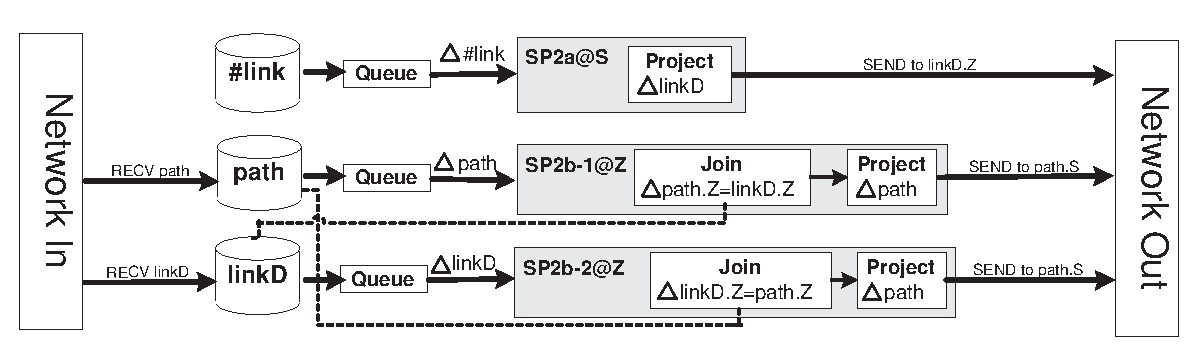
\epsfig{file=images/dataflow1.eps, width=5in}
\caption{\label{Dataflow1}\emph{\small Rule strands for the distributed
    version of SP2 after localization in \Sys.}}
\end{figure*}                                        

The rewrite is achievable because the $link$ and $path$ predicates,
although at different locations, share a common join address field. 
% Based
% on Definition~\ref{def:topRestricted}, we note that all
% link-restricted rules are localizable. 
In Algorithm~\ref{alg:ruleLocal}, we summarize the general rewrite
technique for an input set of link-restricted rules R. In the
pseudocode, for simplicity, we assume that the location specifiers of all the body
predicates are sorted (@S followed by @D); this can be done as a
preprocessing step. The algorithm as presented here assumes that all links are
bidirectional, and may add a \link(@D,@S) to a rewritten rule to
allow for backward propagation of messages.

\vspace{2pt}
{\scriptsize
\begin{Algorithm}[ht]
  \begin{programbox}
    \PROC |RuleLocalization| (R)
     \WHILE \exists | rule r |\in R|: |h(@L,...) :- |\link(@S,@D,...),|
     |\manyquads p|_{1}|(@S,..),..,p|_{i}|(@S,...),|
     |\manyquads p|_{i+1}|(@D,...),..,p|_{n}|(@D,..)| 
%     |\manyquads | \wedge | (| @L=@S | | \vee | | @L=@D )
            R.remove(r)	   
	    R.add(hS(@S,@D,..) :- |\link(@S,@D,..),..,p|_{i}|(@S,..).)|
	    R.add(hD(@D,@S,..) :- hS(@S,@D,..).)
	    \IF @L=@D 
	    \THEN R.add(|h(@D,..) :- hD(@D,@S,..),|
            |\manyquads p|_{i+1}|(@D,..),..,p|_{n}|(@D,..).|)
	    \ELSE R.add(|h(@S,..) :- \link(@D,@S),hD(@D,@S..),|
               |\manyquads p|_{i+1}|(@D,..),..,p|_{n}|(@D,..).|) 
%	       \IF \link.bidirectional
%	       | |\ELSE
%	       error(``illegal rule'')	       
%	       \FI
%            \FI
%     \END
%    \END      
\end{programbox}
\caption{Rule Localization Rewrite}
\label{alg:ruleLocal}
\end{Algorithm}
}
\vspace{2pt}

\begin{Claim}\label{claim:ruleLocal} Every link-restricted \Dlog program, when rewritten using
  Algorithm~\ref{alg:ruleLocal}, produces an equivalent program where
  the following holds:
\begin{CompactEnumerate}
\item The body of each rule can be evaluated at a single node.
\item The communication required to evaluate a rule is limited to
	sending derived tuples over links from a link relation.
\end{CompactEnumerate}
\end{Claim}

The equivalence statement in the above claim can be easily shown,
by examining the simple factoring of each removed rule into two parts. The
remainder of the claim can be verified syntactically in the added rules.
% 
%   because the algorithm generates rewritten
% rules whose body predicates have the same location specifier, and all
% non-local rules generates a tuple that is communicated forwards
% (\link(@S,@D)) or backwards (\link(@D,@S)) based on the input link
% predicate of the input rule. 


Returning to our example, after rule localization we perform the %
semi-\naive rewrite, and then generate the rule strands shown in
Figure~\ref{Dataflow1}.  Unlike the centralized strand in
Figure~\ref{Dataflow}, there are now three rule strands. The extra two
strands ({\em SP2a@S and SP2b-2@Z}) are used as follows. Rule strand
{\em SP2a@S} sends all existing links to the destination address field
as $linkD$ tuples.  Rule strand {\em SP2b-2@Z} takes the new $linkD$
tuples it received via the network and performs a join operation with
the local $path$ table to generate new paths.


\subsection{Relaxing Semi-\naive Evaluation}
In our distributed implementation, the execution of rule strands can
depend on tuples arriving via the network, and can also result in new
tuples being sent over the network. Traditional
semi-\naive evaluation completely evaluates all rules on a given set of
facts, \ie completes the {\em iteration}, before considering any new
facts.  In a distributed execution environment where
messages can be delayed or lost, the completion of an iteration in the
traditional sense can
only be detected by a consensus computation across multiple nodes,
which is expensive; further,
the requirement that many nodes complete the iteration
together (a ``barrier synchronization'' in parallel computing
terminology) limits parallelism significantly by restricting the rate
of progress to that of the slowest node.

We address this by making the notion of iteration local to a node.  New facts might
be generated through local rule execution, or might be received from another node
while a local iteration is in progress.
We propose and prove correct two variations of semi-\naive iteration
to handle this situation: {\em buffered
  semi-\naive} (BSN) and {\em pipelined semi-naive} (PSN).
  Both approaches extend SN to work in an
  asynchronous distributed setting, while generating the same
results as SN evaluation.
We further prove that these techniques avoid
duplicate inferences, which may result in generating network messages. 


\subsubsection{Buffered Semi-\naive}
{\em Buffered semi-\naive} (BSN) is the standard SN algorithm
described in Figure~\ref{alg:sn} with the following modifications: A node can
start a local SN iteration at any time its local $B_{k}$ buffers are
non-empty. Tuples arriving over the network while an iteration is in
progress are buffered for processing in the next iteration. 

By relaxing the need to run an iteration to global completion, BSN relaxes SN
substantially, by allowing a tuple from a traditional SN iteration to be
buffered arbitrarily, and handled in some future iteration of our choice. 
Consequently, BSN may generate
fewer tuples per iteration, but all results will eventually be
generated. Since BSN uses the basic SN
algorithm, the proof of correctness is straightforward and we omit it
for brevity.

The flexibility offered by BSN on when to process a tuple could also
be valuable outside the network setting, \eg a disk-based hash join
could accumulate certain tuples across iterations, spill them to disk in
value-based partitions, and process them in value batches, rather than
in order of iteration number.  Similar arguments for buffering apply
to other query processing tricks: achieving locality in B-tree
lookups, improving run-lengths in tournament sorts, etc.

\subsubsection{Pipelined Semi-\naive}
As an alternative to BSN, {\em pipelined semi-\naive} (PSN) 
relaxes semi-\naive evaluation to the extreme of processing each
tuple as it is received. This provides opportunities for additional
optimizations on a per-tuple basis, at the potential cost of set-oriented
local processing. New tuples that are generated from the
  semi-\naive rules, as well as tuples received from other nodes,
  are used immediately to compute new tuples 
without waiting for the current (local) iteration to complete. 

\vspace{2pt}
%begin{boxedminipage}{3in}
\begin{Algorithm}[ht]
  \begin{programbox}
    \WHILE \exists Q_{k}.size > 0
     t^{old,i}_{k} \LAR Q_{k}.dequeueTuple()
     \FOREACH | rule strand execution | 
     |\quad | \triangle p^{new,i+1}_{j} :- p_{1},..,p_{k-1},t^{old,i}_{k},p_{k+1},..,p_{n},b_{1},b_{2},...,b_{m}
       |\quad| \FOREACH  t^{new,i+1}_{j} \in \triangle p^{new,i+1}_{j}
         \IF t^{new,i+1}_{j} \notin p_{j} 
	 \THEN p_{j} \leftarrow p_{j} \union t^{new,i+1}_{j}
 	      Q_{j}.enqueueTuple(t^{new,i+1}_{j})
%	 \FI
%     \END      
%     \END
%   \END
\end{programbox}
\caption{Pipelined Semi-\naive (PSN) Evaluation}
\label{alg:psn}
\end{Algorithm}
%end{boxedminipage}
\vspace{2pt}


Algorithm~\ref{alg:psn} shows the pseudocode for PSN. Each tuple, denoted $t$, has a
  superscript ($old$/$new$, $i$) where $i$ is its corresponding iteration
  number in SN evaluation. Each processing step in PSN consists of dequeuing a
  tuple $t^{old,i}_{k}$ from $Q_{k}$ and then using it as input into all corresponding
  rule strands. Each resulting $t^{new,i+1}_{j}$ tuple is pipelined,
  stored in its respective $p_{j}$ table (if a copy is not already there), and enqueued into $Q_{j}$ for further
  processing. Note that in a distributed implementation, $Q_{j}$ can be
  a queue on another node, and the node that receives the new tuple can
  immediately process the tuple after the enqueue into $Q_{j}$. For example, the dataflow in Figure~\ref{Dataflow1}
  is based on a distributed implementation of PSN, where incoming
  $path$ and $linkD$ tuples received via the network are stored locally, and enqueued for
  processing in the corresponding rule strands.

%In
%  the pseudocode, each $Q_{k}$ is first initialized with the set
%  of $p_{k}$ tuples by running all the rules using the base tuples as
%  input. Subsequently, $Q_{k}$ acts as a buffer for new $p_{k}$ tuples. 

To fully pipeline evaluation, we have also removed the distinctions
between $p^{old}_{j}$ and $p_{j}$ in the rules. Instead, a timestamp (or
monotonically increasing sequence number) is added to each tuple at
arrival, and the join operator matches each tuple only  
with tuples that have the same or older timestamp. This allows processing of tuples immediately upon
arrival, and is natural for network message handling. This represents
an alternative ``book-keeping'' strategy to the rewriting used in SN to ensure no
repeated inferences. Note that the timestamp only needs to be assigned
locally, since all the rules are localized. 

While PSN enables fully pipeline evaluation, it is worth noting that PSN
can allow just as much buffering as BSN with the additional flexibility
of full pipelining.
%and also allows us to process the join operations on
%sets of tuples. 

%increasing sequence number (or timestamp) to each new tuple 
%prior to
%input to each join operator. Each tuple is then %


%Pipelining non-linear rules with multiple recursive predicates raises the complication of introducing
%duplicate inferences. Consider the following rule with $n$ recursive predicates and
%$m$ base predicates\\
%\noindent {\bf NL1:} $p :- p_{1}, p_{2}, ..., p_{n}, b_{1}, b_{2}, ..., b_{m}$

%In PSN evaluation, there are $n$ semi-\naive rules generated, one for
%each recursive predicate. For the $k^{th}$ recursive predicate, we
%define the {\em $k^{th}$ semi-\naive rule} as follows:\\
%\noindent {\bf NL1-k:} $\triangle$$p^{new} :- p_{1}, ..., \triangle$$p_{k}^{old}, ...,
%p_{n}, b_{1}, b_{2}, ..., b_{m}$

%Duplicates can arise when $t_{j} \in p_{j}$ and $t_{k} \in p_{k}$ are
%derived simultaneously. Based on the PSN algorithm, they are stored in
%their respective queues $Q_{j}$ and $Q_{k}$. When tuple $t_{j}$ is
%dequeued from $Q_{j}$, the $j^{th}$ rule is executed using the pair $t_{j}$
%and $t_{k}$ as inputs. Similarly, when tuple $t_{k}$ is dequeued, the
%pair is again used
%as input to the $j^{th}$ rule. %This results in repeated inferences.
 
In Appendix~\ref{appendix:pipeline}, we prove that PSN generates the same results as SN,
and does not repeat any inferences.
Let $FP_{S}(p)$ and $FP_{P}(p)$ denote the result set for $p$ for
using SN and PSN respectively. We show that:

\vspace{1pt}
\noindent{\bf Theorem~\ref{theorem:nonLinearEq}: } {\em $FP_{S}(p)=FP_{P}(p)$}\\
\noindent{\bf Theorem~\ref{theorem:dupnl}: } {\em There are no
  repeated inferences in computing $FP_{P}(p)$.} 
\vspace{1pt}

In order to compute rules with aggregation (such as SP3), we utilize incremental
fixpoint evaluation techniques~\cite{rossAggregate} that are amenable to
pipelined query processing. These techniques can compute {\em monotonic
  aggregates} such as $min$, $max$ and $count$
incrementally based on the current aggregate and each new input tuple. 
We omit the details for lack of space.



% for a general
%  semi-\naive rule  $\triangle$p$^{new,i+1}_{j}$ :-
%  $p_{1},..,p_{k-1},t^{old,i}_{k},p_{k+1},..,p_{n},b_{1},b_{2},...,b_{m}$. 

%The pseudocode above enforces tuple-at-a-time evaluation,
%which is computationally inefficient. As an optimization, we can flush
%the queue as before to perform set operations, and pipeline any
%generated tuples to their respective queues. 
%However, care has to be
%  taken to ensure that the iteration number is maintained correctly,
%  since the dequeued set may include tuples with different iteration
%  numbers. 




%However, enforcing the FIFO ordering in a queue is also necessary when
%  base tables are updated (Section~\ref{dynamic}).  

%In a distributed implementation of PSN, the queue ($Q$) corresponds to
%the input queue to the rule strand, and each node running the rule strand
%maintains its own separate queue. Hence, each $t^{new, i+1}_{1}$ tuple
%  generated can be inserted into a queue at another node.

%To illustrate PSN evaluation using the rule strands in Figure~\ref{Dataflow1}, we step through the
%communication necessary for the computing the path tuple 
%$p({\bf a},c,b,[a,c,b],2)$ for node {\em a} in Figure~\ref{SP
%  example}: 

%\vspace{1pt}

%\noindent {\bf $1^{st}$ iteration:} Node {\em a} sends
%  $link\_d({\bf a},c,1)$ to {\em c} ({\em rule strand SP2a@a}).

%\vspace{1pt}
%\noindent {\bf $2^{nd}$ iteration:} Node {\em c} receives
%  $link\_d({\bf c},a,1)$ and uses this tuple to 
%  $link\_d$ tuple is used to
%  perform the join ($\bowtie$) with
%  $path({\bf c},b,b,[c,b],1)$ to produce $path({\bf a},c,b,[a,c,d],2)$, which is sent back
%  to node {\em a} ({\em rule strand SP2b-2@c}). 

%\vspace{1pt}

%An optimization that we will explore later is a slight variant,
%known as {\em periodic pipelined} semi-\naive evaluation, where there is a fixed time-interval
%between iterations, and new tuples are processed in a set-oriented fashion.

%\subsubsection{PSN for Linear Rules}
%Consider the following semi-\naive rewritten rule from
%Section~\ref{sec:queryPro}:\\ 
%\noindent{\bf LR1a:} $\triangle$p$^{new}$ :- $\triangle$p$^{old}_{1}$,
%$b_{1}, b_{2}, ..., b_{m}$, where $p_{1}$ is a recursive predicate. 

%\vspace{2pt}
%\noindent{\bf Theorem~\ref{theorem:nseqpsn}: } {\em $FP_{S}(p) =
%FP_{P}(p)$.}\\
%\noindent{\bf Theorem~\ref{theorem:psnnodups}} {\em There are no
%  repeated inferences in computing $FP_{P}(p)$.} 
%\vspace{2pt}

%\subsubsection{PSN for Non-Linear Rules}



%As an optimization to pipelined evaluation, we can execute each rule strand periodically, by
%buffering up events in the queue, and then processing all events when a
%rule strand is activated. This is the pipelined semi-\naive evaluation
%described earlier.




\section{Use Cases}

In the past three years since the introduction of declarative
networking and the release of the \Pitu~\cite{p2} and DSN~\cite{dsn}
declarative networking systems, several applications have been
developed. We describe two of the original use cases that motivated
our work and drove several of our language and system designs: {\em
  safe extensible routers} and {\em overlay network development}.

%~\cite{mobiarch}, ~\cite{meld}.~\cite{Belaramani2009}, ~\cite{shenker}, 
%~\cite{SinghNSDI08}, ~\cite{declarativeSensors,chu07,chu09},
%~\cite{mosaicConext},~\cite{presto08}, 

\subsection{Declarative Routing}

The Internet's core routing infrastructure, while arguably robust and
efficient, has proven to be difficult to evolve to accommodate the
needs of new applications. Prior research on this problem has included
new hard-coded routing protocols on the one hand, and fully extensible
Active Networks on the other. {\em Declarative
  routing}~\cite{declareRoute} explores a new point in this design
space that aims to strike a better balance between the extensibility
and robustness of a routing infrastructure.

With declarative routing, a routing protocol is implemented by writing
a simple query in \Dlog, which is then executed in a distributed
fashion at some or all of the nodes. Declarative routing can be viewed
as a restrictive instantiation of Active Networks for the control
plane, which aims to balance the concerns of expressiveness,
performance and security, properties which are needed for an
extensible routing infrastructure to succeed.

Security is a key concern with any extensible system particularly when
it relates to the consumption of resources due to extensions.  \Dlog
is amenable to static analysis due to its connections to Datalog. {\em
  Pure} Datalog (without any negation, aggregation or function symbols) has
polynomial time and space complexities in the size of the
input~\cite{alicebook}. This property provides a natural bound on the
resource consumption. However, many extensions of Datalog (including
\Dlog) augment the core language in various ways,
extending its polynomial complexity.

Fortunately, static analysis tests have been developed to check for
the termination of an augmented Datalog query on a given
input~\cite{krs}. In a nutshell, these tests identify recursive
definitions in the query rules, and check whether these definitions
terminate. Examples of recursive definitions that terminate are ones
that evaluate monotonically increasing (decreasing) predicates whose
values are upper (lower) bounded. Moreover, the declarative framework is
amenable to other verification techniques, ranging from theorem
proving~\cite{dnv}, model checking~\cite{card}, and runtime
verification~\cite{singhEurosys}.



%Runtime verification~\cite{singhEurosys} is a mechanism for checking
%at runtime that a system does not violate expected properties.  Since
%declarative networks utilize a distributed query engine to execute its
%protocols, these checks can be expressed as {\em monitoring
%  queries}~\cite{singhEurosys} in \Dlog.  Examples include queries for
%monitoring for inconsistent routing or structural property violations
%of networks.


%\reminder{Safety. Talk about model checking~\cite{card}, mechanized theorem
%provers~\cite{dnv}, synthesizing verified specifications~\cite{tpdn},
%etc.}

\Dlog can express a variety of well-known routing protocols (e.g.,
distance vector, path vector, dynamic source routing, link state,
multicast) in a compact and clean fashion, typically in a handful of
lines of program code. Moreover, higher-level routing concepts (e.g.,
QoS constraints) can be achieved via simple modifications to these
queries. Finally, writing the queries in \Dlog illustrates surprising
relationships between protocols.  For example, we have shown that
distance vector and dynamic source routing~\cite{dsr} differ only in a
simple, traditional query optimization decision: the order in which a
query's predicates are evaluated.

To limit query computation to the relevant portion of the network, we
use a query rewrite technique, called {\em magic sets
  rewriting}~\cite{oldMagic}. Rather than reviewing the Magic Sets
optimization here, we illustrate its use in an example: by modifying
rules \nd{sp1-sp4} from the path-vector program, the following computes only
paths limited to sources/destinations in the
\nd{magicSrc}/\nd{magicDst} tables respectively.

\begin{NDlog}
sp1-sd pathDst(@D,S,D,P,C) :- magicSrc(@S), link(@S,D,C),
          P = f\_concatPath(link(@S,D,C), nil). 
sp2-sd pathDst(@D,@S,@Z,P,C) :- pathDst(@Z,@S,Z1,P1,C1),
          link(@Z,@D,C2), C := C1 + C2, 
          P = f\_concatPath(P1,link(@Z,D,C2)).
sp3-sd spCost(@D,S,min<C>) :- magicDst(@D), pathDst(@D,S,Z,P,C).
sp4-sd shortestPath(@D,S,P,C) :- spCost(@D,S,C),
           pathDst(@D,S,Z,P,C).
\end{NDlog}

Our evaluation results~\cite{declareRoute} based on running
declarative routing protocols on PlanetLab and in a local cluster show
that when all nodes issue the same query, the query execution has
similar scalability properties as the traditional distance vector and
path vector protocols. For example, the convergence latency for the
path-vector program is proportional to the network diameter, and
converges in the same time compared to the path vector
protocol. Second, the per-node communication overhead increases
linearly with the number of nodes. This suggests that our approach
does not introduce any fundamental overheads. Moreover, when there are
few nodes issuing the same query, query optimization and work-sharing
techniques can significantly reduced the communication overhead.

One promising direction stems from our surprising observation on the
synergies between query optimization and network routing: a wired
protocol such as the distance-vector protocol can be translated to a
wireless protocol by applying the standard database optimizations of
magic sets rewrite and predicate reordering.  More complex applications of 
query optimization have begun to pay dividends in research research, synthesizing new hybrid protocols from traditional building blocks~\cite{chu09,chuthesis}
Given the proliferation
of new routing protocols and a diversity of new network architecture
proposals, the connection between query optimizations and network
routing suggests that query optimizations may help us inform new
routing protocol designs and allow the hybridization of protocols
within the network.

%due to a wide range of
%variability in network connectivity and also a wide range of data
%traffic patterns, a {\it one-size-fits-all} routing algorithm does not
%exist.  







%\jmh{We need to highlight the biggest nugget here: flexibility between DVR and DSR, the ``upleveling'' of protocol design to query optimization.}





\subsection{Declarative Overlays}
%\petros{Get rid of this, doesn't add much.}
%\reminder{To be fixed}

In declarative routing, we demonstrated the flexibility and
compactness of \Dlog for specifying a variety of routing protocols.
In practice, most distributed systems are much more complex than
simple routing protocols; in addition to routing, they typically also
perform application-level message forwarding and handle the formation
and maintenance of a network as well.

\eat{ All large-scale distributed systems inherently use one or more
  application-level overlay networks as part of their operation.  In
  some cases, the overlay is prominent: for example, file-sharing
  networks maintain neighbor tables to route queries.  In other
  systems, the overlay or overlays may not be as explicit: for
  example, Microsoft Exchange email servers within an enterprise
  maintain an overlay network among themselves using a link-state
  algorithm over TCP for routing mail and status messages.}

In our subsequent work on {\em declarative
  overlays}~\cite{declareOverlays}, we demonstrate the use of \Dlog to
implement practical application-level overlay networks. In declarative
overlays, applications submit to \Sys a concise \Dlog program which
describes an overlay network, and the \Sys system executes the program
to maintain routing tables, perform neighbor discovery and provide
forwarding for the overlay.

\eat{A typical overlay network consists of three functionalities: 

\begin{itemize}
\item {\bf Routing} involves the computation and maintenance of routing
  tables at each node based on input neighbor tables. This functionality
  is typically known as the {\em control plane} of a network.
\item {\bf Forwarding} involves the delivery of overlay messages along
  the computed routes based on the destination addresses of the
  messages. This functionality is typically known as the {\em
  forwarding} plane of a network.
\item {\bf Overlay formation and maintenance} involves the process of
  joining an overlay network and maintaining the neighbor set at each
  node. The selected neighbors are used as input to the control plane
  for route computations.
\end{itemize}}

In declarative routing, \Dlog programs are used solely for programming
the control plane. Hence, all routing examples consist of \Dlog rules
that compute routes based on input links. On the other hand, in
declarative overlays, the \Sys system resides at the application
level, and all messages are routed via the default Internet
routing. Here, \Dlog programs implement the additional functionalities
of neighbor discovery, maintenance, and message forwarding. 

These programs are more complex due to the handling of message
delivery, acknowledgments, failure detection and timeouts required by
the additional functionalities. The programs also heavily utilize
soft-state data and soft-state rules.  Despite the increased
complexity, we demonstrate that our \Dlog programs are significantly
more compact compared to equivalent C++ implementations. For instance,
the use of \Dlog for expressing two complex overlay networks, namely
the Narada mesh formation and a full-fledged implementation of the
Chord distributed hash table in \PNaradaLines and \PChordLines rules
respectively. 

In the case of the Chord DHT, there are rules for performing various
aspects of Chord, including initial joining of the Chord network,
Chord ring maintenance, finger table maintenance, recursive Chord
lookups, and failure detection of neighbors. The detailed Chord
specifications are available in \cite{boonThesis}.

We note that our Chord implementation is roughly two orders of
magnitude less code than the original C++ implementation. This is a
quantitative difference that is sufficiently large that it becomes
qualitative: in our opinion (and experience), declarative programs
that are a few dozen lines of code are markedly easier to understand,
debug and extend than multi-thousand-line imperative programs.
Moreover, we demonstrate in ~\cite{boonThesis,declareOverlays} that
our declarative overlays achieve the expected high-level properties of
their respective overlay networks for both static and dynamic
networks. For example, in a static network of up to $500$ nodes, the
measured hop-count of lookup requests in the Chord network conformed
to the theoretical average of $0.5 \times log_{2}N$ hops, and the
latency numbers were within the same order of magnitude as published
Chord numbers.



 





\eat{
\reminder{Describe Chord in 41 lines briefly. How many rules for doing
  what. Show the recursive lookup rules. }

\reminder{Show the lookup rules of Chord}

In this section, we focus on measuring the full Chord DHT specification
in Appendix~\ref{sec:appendixExamples:chordOverlog}. Chord is a good
stress test of our architecture, being relatively complex compared to
other overlay examples like gossip and end-system multicast.  Chord also
has the advantage of being well-studied. Our \Sys-Chord deployment on
the Emulab testbed~\cite{emulab} consists of $100$ machines executing up
to $500$ \Sys-Chord instances ($5$ \Sys processes running on each Emulab
machine). We utilize the same network topology as the Narada
experiment. Since we are running up to $5$ \Sys processes per Emulab
node, we selected Emulab machines with newer hardware (64-bit Xeon 3000
series with $2$ GB memory) to run our experiments.

\begin{figure*}[ht]
\centering
 \begin{minipage}{.3\linewidth}
  \begin{center}
    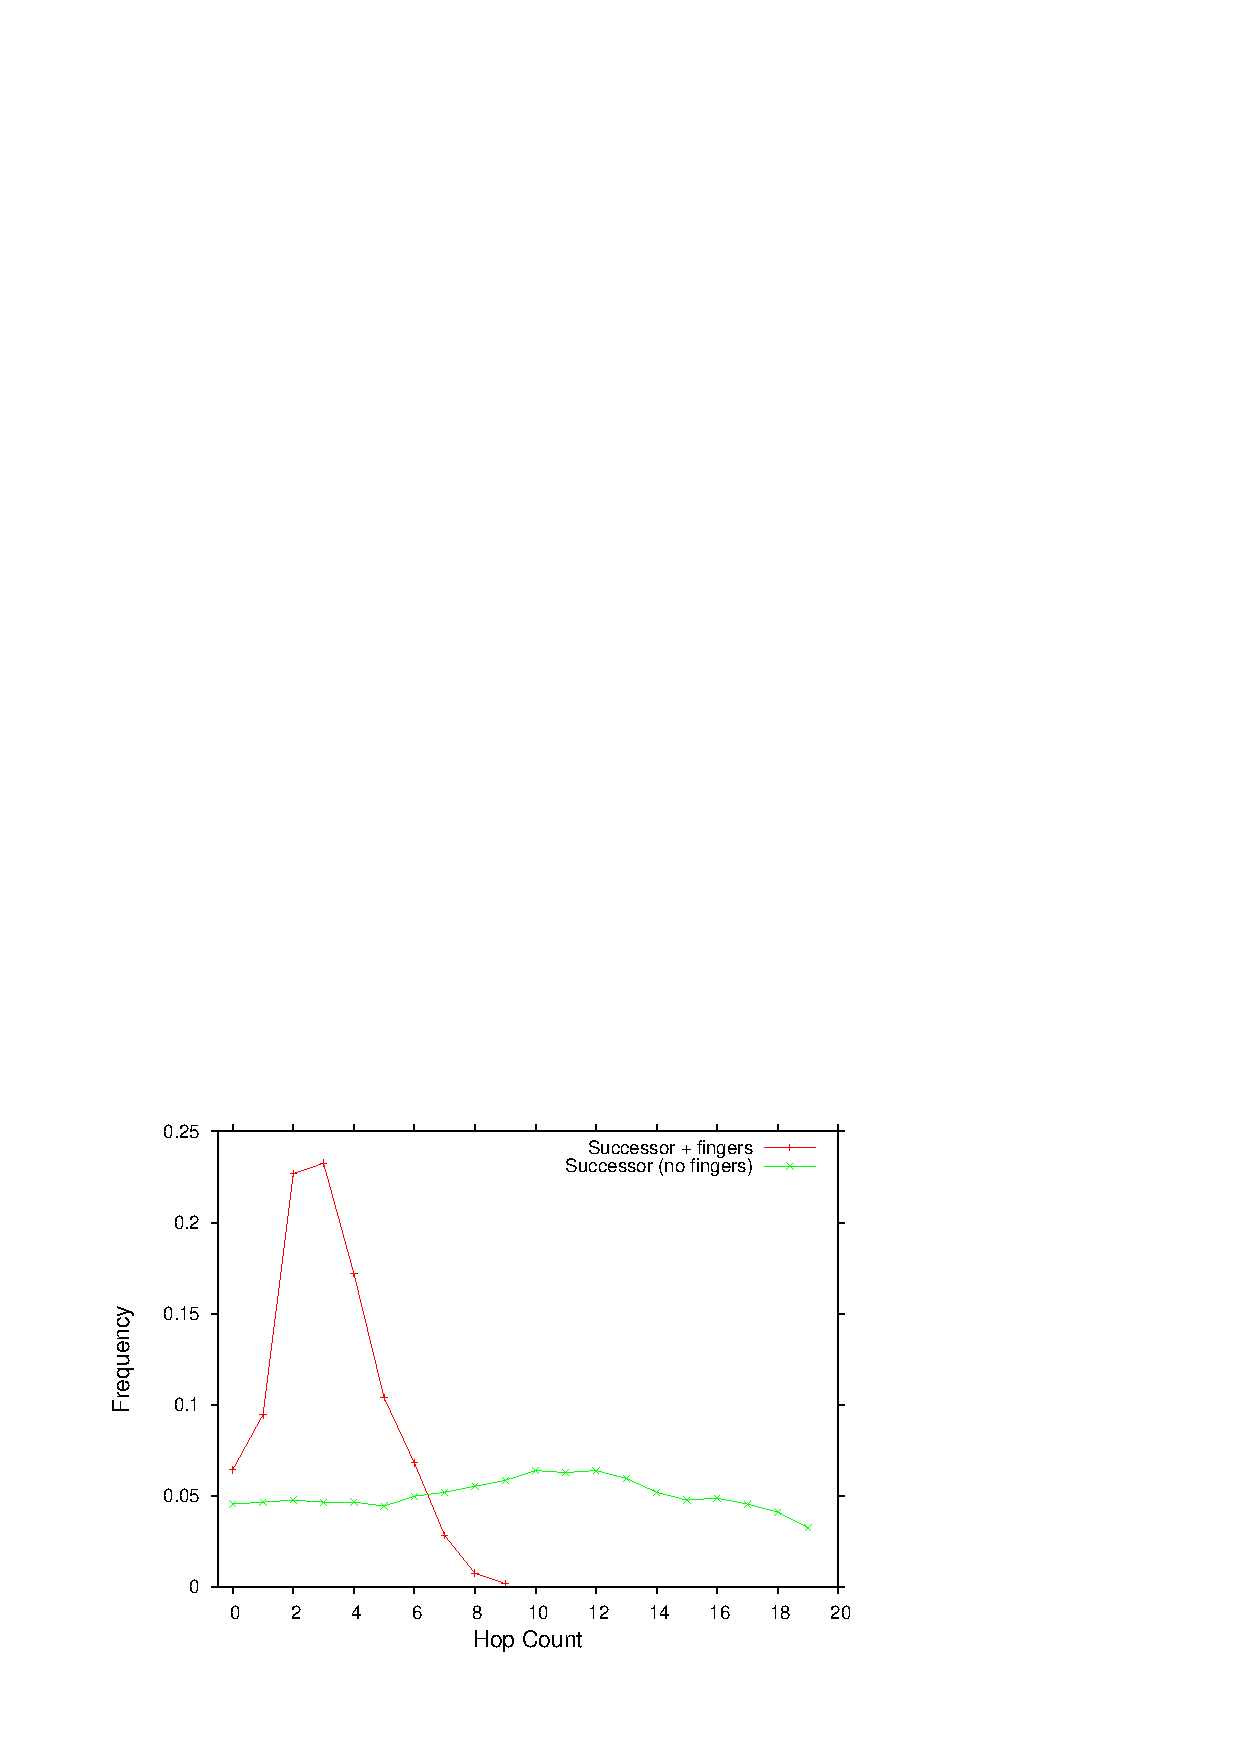
\includegraphics[width=2in]{graphs/overlays/hop_lookup.pdf}
    \caption{{\small Hop-count distribution for lookups.}\label{chord-hop}}
 \end{center}
%\end{figure}
\end{minipage}
\hfill
 \begin{minipage}{.3\linewidth}
%\begin{figure}[ht]
  \begin{center}
    \includegraphics[width=2in]{graphs/overlays/noChurnBW.pdf}
    \caption{{\small Maintenance traffic for different network sizes.}\label{chord-bw}}
  \end{center}
%\end{figure}
 \end{minipage}
\hfill
 \begin{minipage}{.3\linewidth}
%\begin{figure}[ht]
  \begin{center}
    \includegraphics[width=2in]{graphs/overlays/noChurnLatencyCDF.pdf}
    \caption{{\small CDF for lookup latency.}\label{chord-latency}}
  \end{center}
 \end{minipage}
\end{figure*}

%OP\subsubsection{Static Network Validation}

In our first round of experiments, we validate the high-level
characteristics of the Chord overlay. We generate a uniform workload
of DHT ``lookup'' requests to a static set of nodes in the overlay,
with no nodes joining or leaving.  This is somewhat unrealistic but it
allows us to ensure we are achieving the static properties of
Chord. In each experiment, we start a landmark node, and have all
other nodes join the landmark node at regular intervals. Once all the
nodes have joined the Chord overlay, we issue lookups every $15$
seconds simultaneously (with the same lookup key $K$) from $10$ nodes.

Figure~\ref{chord-hop} shows the hop-count distribution for our
workload.  Except for a few outliers, $99\%$ of all lookups complete
within $10$ hops. The average hop count of lookups are $3.3$, $4.0$ and
$4.5$ for node sizes of $100$, $300$ and $500$ respectively,
approximating the theoretical average of $0.5 \times log_{2}(N)$, where $N$ is
the number of nodes.  

Figure~\ref{chord-latency} shows the CDF of lookup latencies for
different network sizes.  As expected, the average latency increases in
proportion to the average lookup hop count for each network size. On a
$500$ node static network, $99\%$ of all lookups complete in less than
$3.4$ seconds. The average (median) latencies are $0.81$ seconds ($0.72$
seconds), $0.92$ seconds ($0.82$ seconds) and $1.09$ seconds ($0.98$
seconds) for node sizes of $100$, $300$ and $500$ respectively. Our
average and median latency numbers are within the same order of
magnitude as the published numbers~\cite{chord} of the MIT Chord
deployment. 

In addition to achieving expected latency numbers, our lookups are also
``correct''. All lookup requests return successfully with the lookup
requests. In addition, all lookups achieve $100\%$ consistency, where
all lookup requests for the same key issued from different nodes return
identical results.

\begin{figure}[ht]
  \begin{center}
    \includegraphics[width=3in]{graphs/overlays/bw.pdf}
    \caption{{\small Per-node Bandwidth (KBps) over time (s).}\label{chord-bw}}
  \end{center}
% \end{minipage}
\end{figure}


Figure~\ref{chord-bw} shows the per-node bandwidth (KBps) consumption
over time (in seconds) for a static \Sys-Chord network where fingers are
fixed every $10$ seconds, and ring stabilization (exchange of successors
and predecessors among neighbors) happen every $10$ seconds. Each node
periodically send ping messages to neighbors every $3$ seconds. After an
initial linear increase in bandwidth as nodes join the Chord ring, the
bandwidth utilization stabilizes at $0.34$ KBps, well within the
published bandwidth consumption of $1$ KBps~\cite{bamboo} of other high
consistency and low latency DHTs.
}



%\subsection{Other Use Cases}


\section{Conclusion}
In Jim Gray's Turing Award Lecture in 1998~\cite{grayturing}, one of
his grand challenges was the development of ``automatic
programming'' techniques that would be (a) $1000\times$ easier for people to use, (b) directly compiled into working code, and (c) suitable for
general purpose use.  
% As of that time, Gray noted that automatic
% programming had been achieved only in a few domain-specific cases.
Butler Lampson reiterated the first two points in a subsequent invited article, but suggested that 
they might be more tractable in domain-specific settings~\cite{lampsonjacm}.  

Declarative Networking has gone a long way towards Gray's vision, if only in the domain of network protocol implementation.  On multiple occasions we have seen at least two orders of magnitude reduction in code size, with the reduced linecount producing qualitative improvements.  In the case of Chord, a multi-thousand line C++ library was rewritten as a declarative program that fits on a single sheet of paper -- a software artifact that can be studied and holistically understood by a programmer in a single sitting.  

We have found that a high-level declarative language not only simplifies a programmer's work, but re-focuses the programming task on appropriately high-level issues. For example, our work on declarative routing concluded that discussions of routing in wired vs.\ wireless networks should not result in different protocols, but rather in different compiler optimizations on the same simple declaration, with the potential to be automatically blended into new hybrid strategies as networks become more diverse~\cite{sigcomm05, ipsn09}.  This lifting of abstractions seems well suited to the increasing complexity of modern networking, introducing software malleability by minimizing the affordances for over-engineering solutions to specific settings.

Since we began our work on this topic, there has been increasing evidence that declarative, data-centric programming has much broader
applicability. Within the networking domain, we have expanded in
multiple directions from our initial work on routing, to encompass
low-level network issues at the wireless link layer~\cite{sensys07} to
higher-level logic including both overlay
networks~\cite{sosp05,sensys07} and applications like code
dissemination, object tracking, and content
distribution~\cite{sensys07,ipsn09}.  Meanwhile, a
variety of groups have been using declarative programming ideas in
surprising ways in many other domains. We briefly highlight two of our own follow-on
efforts:

\begin{itemize}

\item {\bf Secure Distributed Systems:} Despite being developed
independently by separate communities, logic-based security
specifications and declarative networking programs both extend Datalog
in surprisingly similar ways: by supporting the notion of context
(location) to identify components (nodes) in distributed systems.  The
{\em Secure Network Datalog}~\cite{decsec} language extends \Dlog with
basic security constructs for implementing secure distributed systems,
which are further enhanced with type checking and meta-programmability
in the LBTrust~\cite{lbtrust} system for supporting various forms of
encryption/authentication, delegation, for distributed trust
management. 

\item {\bf BOOM: Data-Centric Datacenter Programming}
The BOOM project is exploring the use of declarative languages in the 
setting of Cloud Computing, which currently provide developers with a distributed system and a sequential programming model.  As a counter-example, we used \Overlog as the basis for reimplementing a standard analytics stack for datacenters: the Hadoop File System (HDFS) and MapReduce infrastructure.  Our resulting system is API-compatible with Hadoop, with performance that is equivalent or better.  The high-level \Overlog specification of key Hadoop internals enabled a group of 4 graduate students to quickly add sophisticated distributed features to the system that are not in Hadoop:  hot standby master nodes supported by MultiPaxos consensus, simple scaleout of (quorums of) masters via data partitioning, and simple implementations of new scheduling protocols and query processing strategies~\cite{boom}.  
\end{itemize}

In addition to these two bodies of work, others have successfully
adopted concepts from declarative networking, in the areas of
mobility-based overlays, adaptively hybridized mobile ad-hoc
networks, overlay network composition, sensor networking, fault-tolerant
protocols, network configuration, replication systems, distributed machine 
learning algorithms, and robotics.  
Outside the realm of networking and distributed systems, 
there has been an increasing use of declarative languages -- many rooted in Datalog -- to a wide range of problems including natural language processing, compiler analysis, security and computer games.  We maintain a list of related declarative languages and research projects at \link{http://declarativity.net/related}.  

For the moment, these various efforts represent individual instances of Lampson's domain-specific approach to Gray's automatic programming challenge.  In the coming years it will be interesting to assess whether these solutions prove fruitful, and whether it is feasible to go after Gray's challenge directly: to deliver an attractive general-purpose declarative programming environment for a wide range of tasks.


%In our work, certain design patterns have recurred in the cases where
%our code seemed most compact and natural.  The first is our initial
%inuition that because networks are graphs, many network protocols are
%naturally expressed as transitive closures (recursive queries) of the
%graph's edge relation.  The second was the connection between
%asynchronous communication and join: asynchronous dialogs require the
%rendezvous of cached outbound messages with potentially reordered
%responses -- i.e. the join of the request and response ``stream''.  A
%third pattern is that dynamic programming algorithms are neatly
%expressed as recursive queries, a topic that we have exploited in a
%variety of settings not discussed in this paper.


%\subsection{Recent Developments}


%\subsection{Perspectives}


%additional bullet points
%a) The right abstraction: Data-centric programming key for
%distribution/parallelism (e.g. request/response design patterns,
%leveraging MapReduce excitement, fitness to many distributed tasks)
%b) Recursive state: networks, dynamic programming.
%c) Metamodels and metaprogramming
%       - query optimization
%       - static and dynamic testing for bugs and security
%e) Challenges: update/time semantics, integration/boundaries with native
%code, high performance \& multicore
%f) Going mainstream: cloud \& multicore
%g) Network Verification








% The following two commands are all you need in the
% initial runs of your .tex file to
% produce the bibliography for the citations in your paper.
\bibliographystyle{abbrv} % standard abbrv style
\bibliography{biblio}  % substitute the name of 'your' Bibliography here
% You must have a proper ".bib" file
% and remember to run:
% latex bibtex latex latex (in that particular order) in order to resolve all the 'numerical values'
% be they for figures, equation numbers, references, footnotes, etc. etc.
%
\balancecolumns
% That's all folks! % GM Sept. 2008
\end{document}
